\noindent\makebox[.9\paperwidth]{
\noindent
\setlength\arrayrulewidth{4pt}
\begin{tabular}{p{.2\paperwidth}@{}!{\color{goldan-yellow}\vline width 1.5pt}p{.64\paperwidth}}
\hfill\raisebox{-3.5cm}{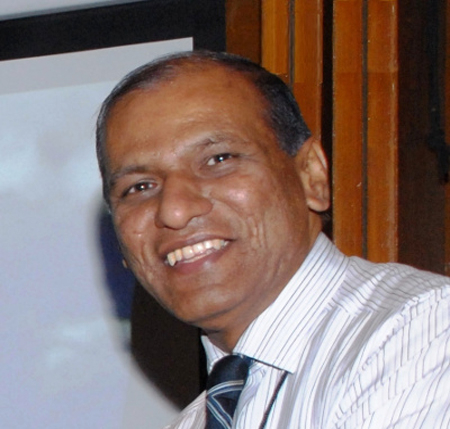
\includegraphics{src/Figures/Ramamurthy.jpg}~~}\newline\newline
\rule{.2\paperwidth}{.4pt}
& This issue of ACC focuses on a technology that is much talked about in recent times not by communication engineers alone but by global political leaders as well – the fifth generation (5G) wireless communication technology. The importance of this technology is evident if one were to consider its impact on billions of users as the services offered in 5G are expected to find wide ranging applications such as vehicular networks, e-health, education, and industrial Internet of Things (IoT) to list a few.  

\bigskip

In the article titled ‘Non-Orthogonal Multiple Access (NOMA)’, the author discusses recently proposed Power Domain NOMA and Code Domain NOMA as techniques to increase the network throughput and to support massive connectivity, which are major requirements in the 5G communication systems. 

\bigskip

Security continues to be a major issue in 5G systems as well. The 3rd Generation Partnership Project (3GPP) defined 5G system envisages fundamental changes on top of its former cellular systems in several design areas including security. In their paper titled ‘xxxxxxx’ the authors discuss the key enhancements specified by the 3GPP for the 5G system, particularly those that differ from the previous 4G system and the rationale for the same.

\bigskip

Some of the technological drivers for 5G include developments in massive MIMO, cognitive radios, millimetre wave communications, network virtualization, software defined networking, etc. An underlying technology that has enabled most of these developments possible is the continued miniaturization of devices in the nano scale regime and the capability to manipulate the matter at these dimensions. This is expected to revolutionize the future systems for computation, storage and perception in the next few decades. In the article titled ‘Nanotechnology and the Future of Computation, Storage and Perception’ the author foresees availability of very powerful artificial intelligence (AI) and machine learning (ML) hardware chips, enabled by the integration of new compute and storage technologies co-existing with a variety of sensors.  

\bigskip

It has been universally accepted that education is a right of every human being is a means towards empowerment. In their article titled ‘Characterization of Technology based Mediations for Navigated Learning’, the authors discuss a new paradigm for learning that aims for a holistic integration of the three independent educational requirements: scalability, personalization and social learning. The authors describe a pedagogic model and a platform for navigated learning.  

\bigskip

In continuation of their series of articles on experiential learning, the authors explain the basics of flow control in client server communication based on TCP and provide experiential learning exercises to help understand its impact on TCP performance.

\bigskip

Hope that all of the above articles are timely and of immense interest to our targeted readers 


\bigskip

\hfill  Dr. N Rama Murthy\hspace{1cm}\,

\vskip 2pt

\hfill Editor\hspace{3.15cm}\,

\end{tabular}
}





